\documentclass[12pt,a4paper]{report}

\usepackage[a4paper,margin=1in]{geometry}
\usepackage{graphicx}
\usepackage{subcaption}
\captionsetup[subfigure]{list=false}
\usepackage{float}
\usepackage{xurl}
\usepackage[hidelinks]{hyperref}
\usepackage{setspace}
\usepackage{tikz}
\usepackage{eso-pic}
\usetikzlibrary{calc}

% ---------- PAGE BORDER ----------
\AddToShipoutPictureBG{%
\begin{tikzpicture}[remember picture,overlay]
\draw[line width=2pt]
($(current page.north west)+(1cm,-1cm)$)
rectangle
($(current page.south east)+(-1cm,1cm)$);
\end{tikzpicture}%
}

\begin{document}

%================================================
% TITLE PAGE
%================================================

\begin{titlepage}
\begin{center}

{\Huge \textbf{INTERNSHIP REPORT}}

\vspace{1cm}

On

\vspace{0.6cm}

{\Large \textbf{Football }}

\vspace{1cm}

By

\vspace{0.5cm}

Ayush Masurkar (TECOC-23)

\vspace{1cm}

Under the guidance of

\vspace{0.6cm}

% LOGO
\includegraphics[width=5cm]{College Logo.png}

\vspace{0.6cm}

Mrs. Ketaki Chinchane

\vspace{1cm}

{
Department of Computer Engineering \\

Pimpri Chinchwad Education Trust’s \\

Pimpri Chinchwad College of Engineering \& Research Ravet, Pune \\

An Autonomous Institute | NBA Accredited (4 UG Programs) | NAAC A++ Accredited | ISO 21001:2018 Certified
}

\vspace{0.5cm}

\textbf{Savitribai Phule Pune University}

\vspace{0.3cm}

\textbf{Academic Year: 2025--2026}

\end{center}
\end{titlepage}

%================================================
% CERTIFICATE PAGE
%================================================

\newpage

\begin{center}

\textbf{Pimpri Chinchwad Education Trust’s}

\vspace{0.2cm}

{\Large \textbf{Pimpri Chinchwad College of Engineering \& Research Ravet, Pune}}

\vspace{0.2cm}

An Autonomous Institute | NBA Accredited (4 UG Programs) | NAAC A++ Accredited | ISO 21001:2018 Certified

\vspace{0.8cm}

\includegraphics[width=4cm]{College Logo.png}

\vspace{0.6cm}

{\Large \textbf{CERTIFICATE}}

\end{center}

\vspace{1cm}

This is to certify that the internship report titled \textbf{“Football ”}, submitted by \textbf{Ayush Masurkar (TECOC-23)}, has been successfully presented as part of the internship seminar in partial fulfillment of the requirements for the Third Year (Computer Engineering). This work has been carried out during the academic year \textbf{2025--2026}.

\vspace{2cm}

Date: 30/03/2026

Place: Ravet

\vspace{3cm}

% ---------- SIGNATURE AREA ----------
\begin{center}
\begin{tabular}{ccc}

\textbf{Mrs. Ketaki Chinchane} &
\textbf{Dr. Vijay A. Kotkar} &
\textbf{Dr. H. U. Tiwari} \\[6pt]

Internship Co-ordinator &
HOD, Computer Department &
Director, PCCOE\&R \\

&
PCCOE\&R &

\end{tabular}
\end{center}

%================================================
% ACKNOWLEDGEMENT
%================================================

\newpage
\begin{center}
{\Large \textbf{ACKNOWLEDGEMENT}}
\end{center}

\vspace{0.5cm}

It gives me great pleasure to present the internship report on \textit{Football }. In preparing this report, many people helped me directly and indirectly.

I am grateful to the faculty members of the Computer Engineering Department for their guidance and support throughout the development of this internship work. I express my sincere gratitude to the Head of Department, Dr. Vijay A. Kotkar, and all the staff members for their cooperation. I am also thankful to my family and friends for their constant encouragement and support.

\vspace{2cm}

Place: Ravet, Pune

Date: 02/04/2026

\vspace{1cm}

\begin{flushright}
Ayush Masurkar \\
TECOC-23
\end{flushright}

%================================================
% TABLE OF CONTENTS
%================================================

\newpage
\tableofcontents

%================================================
% LIST OF FIGURES
%================================================

\newpage
\listoffigures

%================================================
% CHAPTER 1
%================================================

\chapter{Introduction}

\section{Introduction}
In football tournaments and league-style competitions, generating fixtures is one of the most important operational tasks. Organizers must ensure that teams are grouped correctly, schedules remain fair, and every match is clearly defined before an event begins. In small tournaments this process may be manageable by hand, but as the number of teams increases, manual scheduling quickly becomes difficult, repetitive, and error-prone.

Traditional manual methods such as spreadsheet planning or handwritten match tables often introduce avoidable issues, including duplicate pairings, missing matches, uneven group distributions, and confusion during schedule communication. These challenges can affect tournament quality, consume additional time, and create unnecessary stress for coordinators, players, and event managers.

The \textbf{Football } is designed as a practical solution to these problems. It is a web-based application that accepts team names, processes them in a structured way, randomizes group allocation, and generates round-robin fixtures automatically. The generator helps ensure consistency, reduces planning time, and provides a clean output that can be shared immediately.

This internship implementation is developed using \textbf{Next.js}, \textbf{TypeScript}, \textbf{Tailwind CSS}, and \textbf{shadcn/ui}. The logic is organized into reusable utility modules for input parsing, team shuffling, group creation, and fixture generation. The user interface is kept simple and responsive so that the application can be used efficiently on common desktop and laptop environments.

The current workflow follows a two-page approach. The home page is dedicated to team input and fixture generation, while the fixtures page presents the final matchday schedule with grouped matches. Additional controls such as copy and regenerate improve usability and make the tool suitable for real-world event preparation.

Overall, the Football  demonstrates how frontend development and algorithmic thinking can be combined to solve a real scheduling problem in sports management. It also highlights the value of automation in reducing human effort, increasing reliability, and improving the overall planning experience.

\section{Company Details}
\begin{itemize}
    \item \textbf{SkillCraft Technology:}
    Completed a one-month Web Development Internship, focusing on building and deploying web applications.

    \item
    This project was carried out under the Department of Computer Engineering, PCCOE\&R, Pune.
\end{itemize}

\section{Problem Statement}
Tournament organizers often need a fast way to create grouped fixtures from a list of football teams. Manual scheduling can lead to mistakes, imbalance, and wasted time. A simple automated tool is needed to accept team names, create randomized groups of three, and generate all fixtures in a readable format.

\section{Objectives}
The primary objectives of the Football  are as follows:
\begin{itemize}
    \item \textbf{Provide a simple and clear input experience:} The system should allow users to enter team names quickly using comma-separated or line-separated text input without requiring complex formatting.

    \item \textbf{Ensure fairness in team allocation:} The application should randomize team ordering using the Fisher-Yates shuffle so that grouping is unbiased and different schedules can be generated when required.

    \item \textbf{Create balanced groups automatically:} The system should divide teams into groups of three while handling uneven totals in a practical and structured manner.

    \item \textbf{Generate complete round-robin fixtures:} Every team in a group should play every other team once, ensuring no missing pairings and no duplicate match entries.

    \item \textbf{Separate generation and schedule display:} The workflow should keep team entry and fixture display on different pages for better readability and a cleaner user experience.

    \item \textbf{Improve usability through actions:} The application should provide regenerate and copy options so users can quickly reshuffle schedules or share fixture outputs.

    \item \textbf{Handle edge cases safely:} The system should validate empty input, insufficient team count, and invalid values to avoid incorrect schedule generation.

    \item \textbf{Maintain modular and readable code structure:} Core logic should be separated from UI components using utility functions and TypeScript types for easier maintenance and extension.

    \item \textbf{Demonstrate practical internship outcomes:} The project should showcase real-world application of web technologies, algorithm implementation, and user-centric design in a domain-relevant problem.
\end{itemize}

%================================================
% CHAPTER 2
%================================================

\chapter{Methodology / Proposed System}

\section{System Architecture}
The application follows a simple client-side architecture:
\begin{enumerate}
    \item \textbf{Input Collection:} The home page contains a textarea for entering team names and a selector for group size.
    \item \textbf{Input Parsing:} Team names are split using commas or line breaks and trimmed to remove extra spaces.
    \item \textbf{Randomization:} Teams are shuffled using the Fisher-Yates algorithm to produce unbiased random groupings.
    \item \textbf{Grouping:} The shuffled teams are divided into groups of three.
    \item \textbf{Fixture Generation:} A round-robin list of matches is created for every group.
    \item \textbf{Data Sharing:} Generated data is saved in browser storage so it can be loaded on the fixtures page.
    \item \textbf{Display:} The fixtures page reads the saved data and renders the matchday schedule.
\end{enumerate}

\begin{figure}[h!]
    \centering
    \includegraphics[width=0.8\textwidth]{fixture_generator_architecture.png}
    \caption{System architecture of the Football }
\end{figure}

\section{Workflow}
The workflow of the application is as follows:
\begin{itemize}
    \item The user enters team names on the home page.
    \item The application validates the input and checks whether at least two teams are provided.
    \item The teams are shuffled and grouped.
    \item Round-robin fixtures are generated for each group.
    \item The user is redirected to the fixtures page where the full schedule is displayed.
\end{itemize}

\section{Feature Handling}
\begin{itemize}
    \item \textbf{Empty Input:} The application shows a helpful message when no teams are entered.
    \item \textbf{Less Than Two Teams:} Fixture generation is blocked because a match requires at least two teams.
    \item \textbf{Uneven Group Sizes:} The grouping logic balances teams as evenly as possible when the total is not divisible by three.
    \item \textbf{Fixed Group Size:} The interface keeps the group size locked to three teams per group.
\end{itemize}

\section{Algorithms and Technologies Used}

\subsection{Algorithm}
The main algorithm used in the internship work is the \textbf{Fisher-Yates shuffle}, which randomizes the order of the teams. After shuffling, the teams are divided into groups and fixtures are created using a round-robin pairing method.

\subsection{Input Processing}
The input processing steps are:
\begin{itemize}
    \item Split team names by commas or new lines.
    \item Remove extra spaces from each team name.
    \item Filter out empty values.
\end{itemize}

\subsection{Frontend Technology}
\textbf{Next.js} is used for routing and page rendering. The home page contains the generator form, and the fixtures page displays the matchday schedule.

\subsection{Styling}
\textbf{Tailwind CSS} and \textbf{shadcn/ui} are used to create a modern, responsive user interface with cards, buttons, inputs, and textareas.

\subsection{Data Storage}
Generated groups and fixtures are stored in \textbf{localStorage} so the schedule page can load the latest output without a backend.

\subsection{Group Formation Logic}
The grouping logic uses a shuffle step followed by a fixed three-team grouping rule so that the output remains consistent with the current internship configuration.

\subsection{Other Technologies}
\begin{itemize}
    \item \textbf{React:} For reusable user interface components.
    \item \textbf{TypeScript:} For type safety and maintainable code.
    \item \textbf{Lucide React:} For icons used in the interface.
\end{itemize}

%================================================
% CHAPTER 3
%================================================

\chapter{Hardware and Software Requirements}

\section{Frontend Technology}
The application uses a modern frontend stack to provide a smooth user experience. The key features of the interface include simple form input on the home page, route-based navigation, responsive layouts, and interactive controls such as generate, copy, and regenerate buttons on the fixtures page.

\textbf{Installation:}
\begin{verbatim}
npm install
\end{verbatim}

\section{System Setup and Configuration}
To run the internship work environment, follow these steps:
\begin{enumerate}
    \item Install Node.js and the required internship work dependencies.
    \item Start the development server.
    \item Open the home page and enter team names.
    \item Click \textbf{Generate Fixtures} to create and save groups.
    \item View the matchday schedule on the fixtures page.
\end{enumerate}

\section{Hardware Requirements}
The hardware requirements for this internship work are modest and suitable for most systems:
\begin{itemize}
    \item \textbf{Processor:} Intel Core i3 or higher
    \item \textbf{RAM:} Minimum 4GB, 8GB recommended
    \item \textbf{Storage:} At least 1GB of free disk space
    \item \textbf{Operating System:} Windows, macOS, or Linux
    \item \textbf{Browser:} Latest version of Chrome, Firefox, Edge, or Safari
\end{itemize}

\section{Software Requirements}
\begin{itemize}
    \item Node.js 18 or higher
    \item Next.js App Router setup
    \item Tailwind CSS
    \item TypeScript
    \item shadcn/ui components
\end{itemize}

%================================================
% CHAPTER 4
%================================================

\chapter{Result and Conclusion}

\section{Results}
The Football  successfully creates randomized groups and round-robin fixtures from a list of team names. The home page acts as the input and generation screen, while the fixtures page shows the matchday schedule.

\begin{figure}[H]
    \centering
    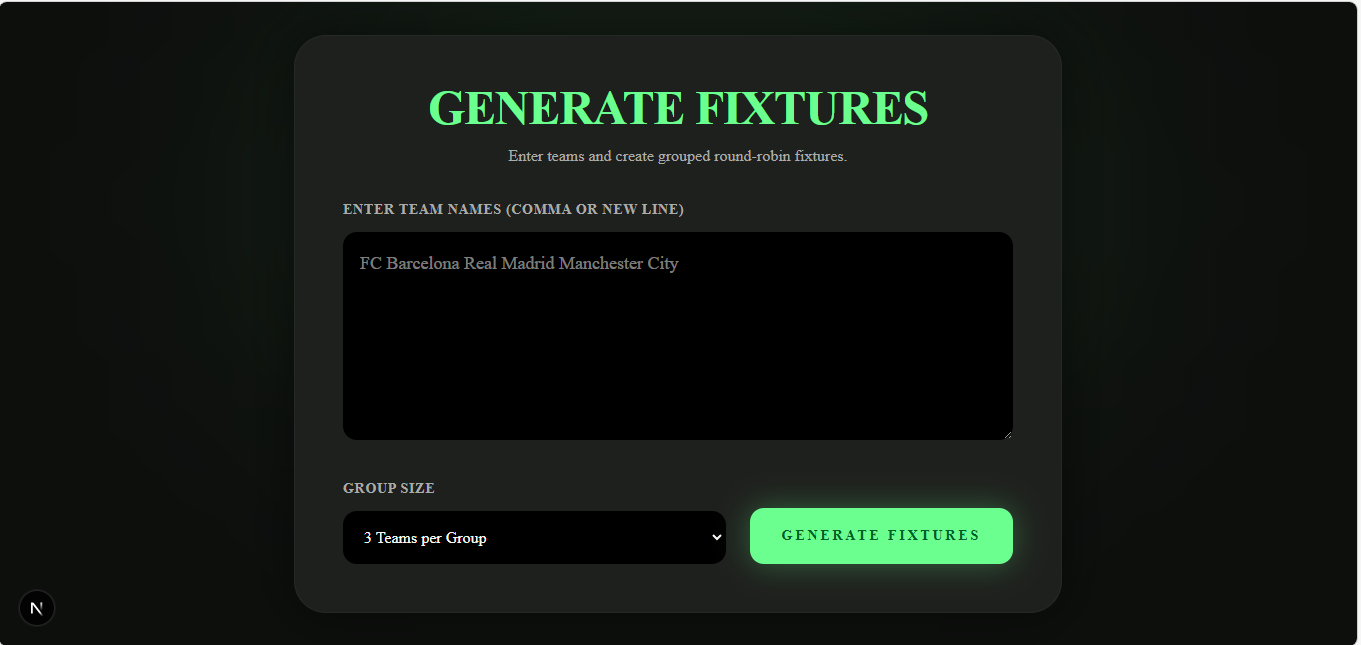
\includegraphics[width=0.92\textwidth]{result1.png}
    \caption{Home page with fixture input form}
\end{figure}

\begin{figure}[H]
    \centering
    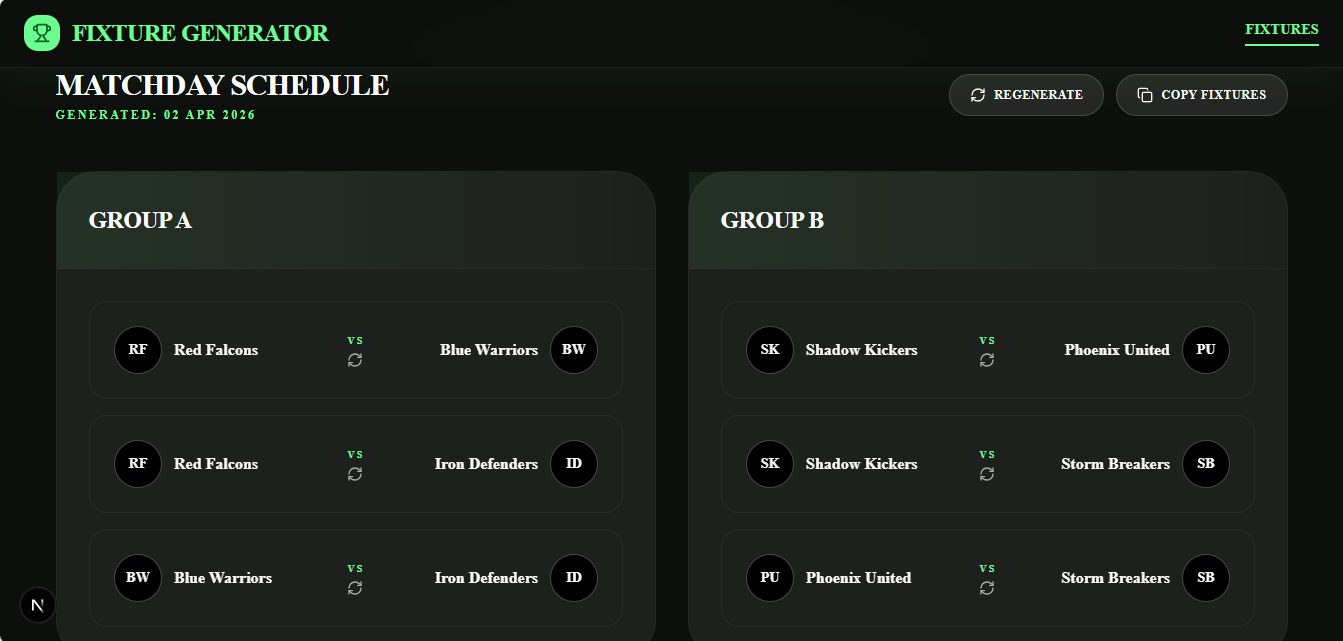
\includegraphics[width=0.92\textwidth]{result2.png}
    \caption{Fixtures page with generated schedule}
\end{figure}

The screenshots above show the home page used for fixture generation and the fixtures page that displays the grouped match schedule.

\section{Conclusion}
The internship work provides a practical and easy-to-use solution for generating football fixtures. It reduces manual effort, improves scheduling speed, and presents the results in a clean modern interface.

\section{Future Scope}
\begin{itemize}
    \item Add support for custom group sizes.
    \item Add home-and-away fixture generation.
    \item Export fixtures as PDF or CSV.
    \item Save schedules in a database for later access.
    \item Add tournament management features such as standings and points tables.
\end{itemize}

\section{References}
\begin{itemize}
    \item Next.js Documentation, \url{https://nextjs.org/docs}
    \item Tailwind CSS Documentation, \url{https://tailwindcss.com/docs}
    \item shadcn/ui Documentation, \url{https://ui.shadcn.com/}
    \item MDN Web Docs, \url{https://developer.mozilla.org/en-US/docs/Web/API/Window/localStorage}
    \item Fisher-Yates Shuffle Reference, \url{https://en.wikipedia.org/wiki/Fisher%E2%80%93Yates_shuffle}
\end{itemize}

%================================================
% CHAPTER 5
%================================================

\chapter{Internship Completion Summary}

\section{Summary}
The Football  internship work is a complete frontend-based scheduling tool that accepts team names on the home page, generates grouped fixtures, and displays the final matchday schedule on a dedicated fixtures page.

\section{Implementation Notes}
The application uses browser storage to preserve generated fixtures between pages. This keeps the implementation simple and avoids the need for a backend server while maintaining the current page flow of the internship work.

\end{document}
